\documentclass[a4paper,11pt, oneside]{article}  % document class
\usepackage{geometry}
\geometry{
	inner=20mm,
	outer=20mm,
	top=30mm,
	bottom=25mm %
	%  heightrounded,
	%  marginparwidth=50pt,
	%  marginparsep=17pt,
	%  headsep=20pt
}
\usepackage[english]{babel}
\usepackage{hyperref}
%pacchetto
\usepackage{import, multicol,lipsum}  % package
\setlength{\columnsep}{1cm}

\usepackage[utf8]{inputenc} % accenti facili
\usepackage[T1]{fontenc}
\usepackage{subcaption}
\usepackage{pifont}
\usepackage{url}
\hypersetup{
	colorlinks=true,
	linkcolor=blue,
	filecolor=magenta,      
	urlcolor=blue
}
\usepackage{graphicx, color, blindtext}
\usepackage{textcomp, makeidx, times}
\usepackage{amsthm, amsmath, amssymb, amsfonts, mathtools} % math
\usepackage[mathscr]{eucal}		
\usepackage[nottoc]{tocbibind} 
\usepackage{pgfplots, parskip}
\usepackage{afterpage, ifthen}
\usepackage{enumitem}
\pgfplotsset{compat=newest}
\usepackage{graphicx} % immagini
\usepackage{wrapfig}
%\graphicspath{ {image/} } % path cartella delle immagini
\usepackage{tikz} %graph
\usetikzlibrary{arrows,automata}
\usetikzlibrary{automata,arrows,positioning,calc,matrix}
\usepackage[linesnumbered,ruled,vlined]{algorithm2e}
\usepackage{booktabs}
\usepackage{colortbl}
\usepackage{siunitx}
\usepackage{tabularx, tabu}
\usepackage{relsize}
\usepackage{makecell, caption, chngcntr}
\usepackage{bbm}
\usepackage{diffcoeff}
\RequirePackage{fix-cm}


%
%____________________________________________________________________________________________________________________________
%____________________________________________________________________________________________________________________________
%____________________________________________________________________________________________________________________________
%____________________________________________________________________________________________________________________________
% INIZIO
\begin{document}
	
	\setcounter{secnumdepth}{2}
	\pagestyle{plain} % stile pagina (header, numerazioni)
	
	\centerline {
\includegraphics[width=2cm]{logo.jpg}}
	\begin{center}
		Università degli Studi di Torino - M.Sc.  in Stochastic and Data Science - A.Y.  2021/2022 \\
		\Large { Final project of Statistical Machine Learning (MAT0043)}
		\line(1,0){450}\\ 
		\vspace{0.4cm} 
		{ \huge \textbf{Gene selection for cancer type classification} }
		\vspace{0.1cm}
		\line(1,0){450} \\
	\end{center}
	
	%____________________________________________________________________________________________________________________________
	%____________________________________________________________________________________________________________________________
	% ABSTRACT
	%From the DepMap Portal website\footnote{DepMap Portal: \url{https://depmap.org/portal/} } we downloaded a dataset containing 1032 cancerous cells whose $\sim 17000$ columns represent the probability that the inhibition of that given gene stops the growth of the cancer.  The label of each cell line refers to the cancer type and is a categorical factor which can assume 10 values: Eye, Gastrointestinal,  Gynecologic,  Musculoskeletal,  Neurological,  Breast,  Head-Neck,  Hematologic,  Genitourinary,  Lung.  The project then focuses on the problem of Genes Selection for Cancer Classification,  i.e.  finding a relatively small number of genes to predict the type of cancer of a given tumorous cell.  To this aim we explored in detail three Features Selection algorithms: Random Forests combined with Feature Importance,  Lasso-SVM and Neural Networks (NN) combined with Permutation Importance.  We repeated these procedures on three distinct classification tasks: blood cancer vs rest,  lung cancer vs rest and multiclass.  Apart from the cases involving lung data,  we achieved satisfying classification accuracies on the whole dataset and we were able to select about 100-200 genes from the starting ~17000 ones.  We then used these features to fit reduced versions of the previous classifiers and obtained classification accuracies which range from $67\%$ to $98\%$.  We then concluded that the possibility of classifying the type of cancer from an extremely reduced numbers of genes depends on the cancer type itself.  In particular,  these methodologies worked incredibly well on blood cancer for which we achieved almost $100\%$ accuracy with the reduced classifier while failed miserably on lung cancer.  
	
	The purpose of our project is to work on a high-dimensional genomics data and find a relatively small number of genes to predict the cancer type of a given tumorous cells. This is known as Genes Selection for Cancer Classification and it is in line with many up-to-date problems of applied medicine. \\
	Our dataset contained $1.032$ cancerous cells and their knock-out probabilities, i.e. the probabilities of stopping the growth of tumour by inhibiting one of the $\sim 17.000$ genes. Each cell line was characterised by one of 10 possible cancer labels: Eye, Gastrointestinal, Gynecologic, Musculoskeletal, Neurological, Breast, Head-Neck, Hematologic, Genitourinary and, finally, Lung. We explored in details three Features Selection algorithms: Random Forests (RF) combined with Feature Importance, Lasso-SVM and Neural Networks (NN) combined with Permutation Importance. We studied two binary classifications (Blood-cancer vs. All, Lung-cancer vs. All) and a multiclass classification. Besides lung models, we achieved satisfying classification accuracies and we were able to select about $100$-$200$ genes from the initial $\sim 17.000$ ones. Models fitted on such genes obtained classification accuracies ranging from $67\%$ to $98\%$. \\
	Therefore, it seems that classifying cancer type from an extremely small set of genes depends on the cancer type itself. These methodologies worked incredibly well on Blood cancer, as we reached almost $100\%$ accuracy with the reduced classifier, whereas failed miserably on Lung cancer.  
	
	
	\section{Introduction}
	Cancer is a complex disease characterized by the uncontrolled growth of abnormal cells anywhere in the body. These abnormal cells are extremely invasive and we usually identify them with the name of their original tissue (for instance, breast cancer, lung cancer,  brain cancer, etc.).  In recent years, medicine has made a great step forward in finding new and efficient therapies for different diseases and cancer is one of them.  In particular,  thanks to numerous advances in technology,  collecting huge amount of data is no longer an issue, so that one can exploit such information to define personalized treatments for patients. In this regards, the DepMap project\footnote{DepMap Portal: \url{https://depmap.org/portal/} } and,  in particular,  the Achilles project\footnote{Achilles Project: \url{https://depmap.org/portal/achilles/} } aim to use genome-wide screens to collect data regarding mutations of cancerous cells,  identify essential genes and report vulnerabilities across hundreds of human cancers.  \\
	
	Many researches are currently using DepMap datasets to identify relatively small sets of genes which are responsible of cancers growth. This procedure is often driven by medical knowledge,  which we do not possess,  together with some rough measures of importance.  Being Maths student,  we instead base our research on statistical models and on the hypothesis that, if a given classifier is able to distinguish different types of cancer, then the most relevant genes are the most important features for that given classifier (the meaning of "important features" will be clarified later). Of course, selecting few truly significant genes has outstanding implications in the medical field: building faster diagnosis tools and synthesising less toxic drugs are only two examples. 
	
	
	\section{Dataset}
	We used two public datasets from the DepMap Portal website\footnote{Download dataset from DepMap:  \url{https://depmap.org/portal/download/}:} :
	\begin{itemize}
		\item[D1] \textit{CRISPR\_gene\_dependency.csv},  which contains $1.032$ cancer cell lines characterised by $17.393$ gene scoring results
		\item[D2] \textit{sample\_info.csv}, which contains cell lines information,  such as primary disease and sample collection site
	\end{itemize}
	Data were collected from real patients and successively processed,  so that element $(i, j)$ of this $(1.032 \times 17.393)$-data frame is the probability that knocking out gene $j$ has a real depletion effect on the $i$-th cell.
	Before proceeding with our analysis, we removed missing values, which affected only 10 rows coming from different tumours, and we looked for weird observation. In particular, we found $2$ "Non-Cancerous" and $6$ "Engineered" cells. The first can be reasonably discarded, whereas the latter requires a little care. Engineered cells are synthetically modified samples in lab and, here, they are manly associated to the Eye sample collection site. We decided to keep them and associate them to the cancer corresponding to their site. \\
	Side note: in general, looking also at the sample collection site do not ease tumour classification. Indeed, metastasis of the original compromised tissue can be found all over the body. \\
	%  In order to work on a labelled datasets and perform classification, we associated the primary disease (i.e. the name of the cancer type) to each cell line performing an inner join of D1 and D2 on the DepMap ID.  Then,  we dedicated ourselves in data cleaning: we removed missing values,  which affected only 10 rows,  and all instances labeled as "Non Cancerous" and "Engineered".  
	
	\begin{wrapfigure}{r}{0.65\textwidth}
		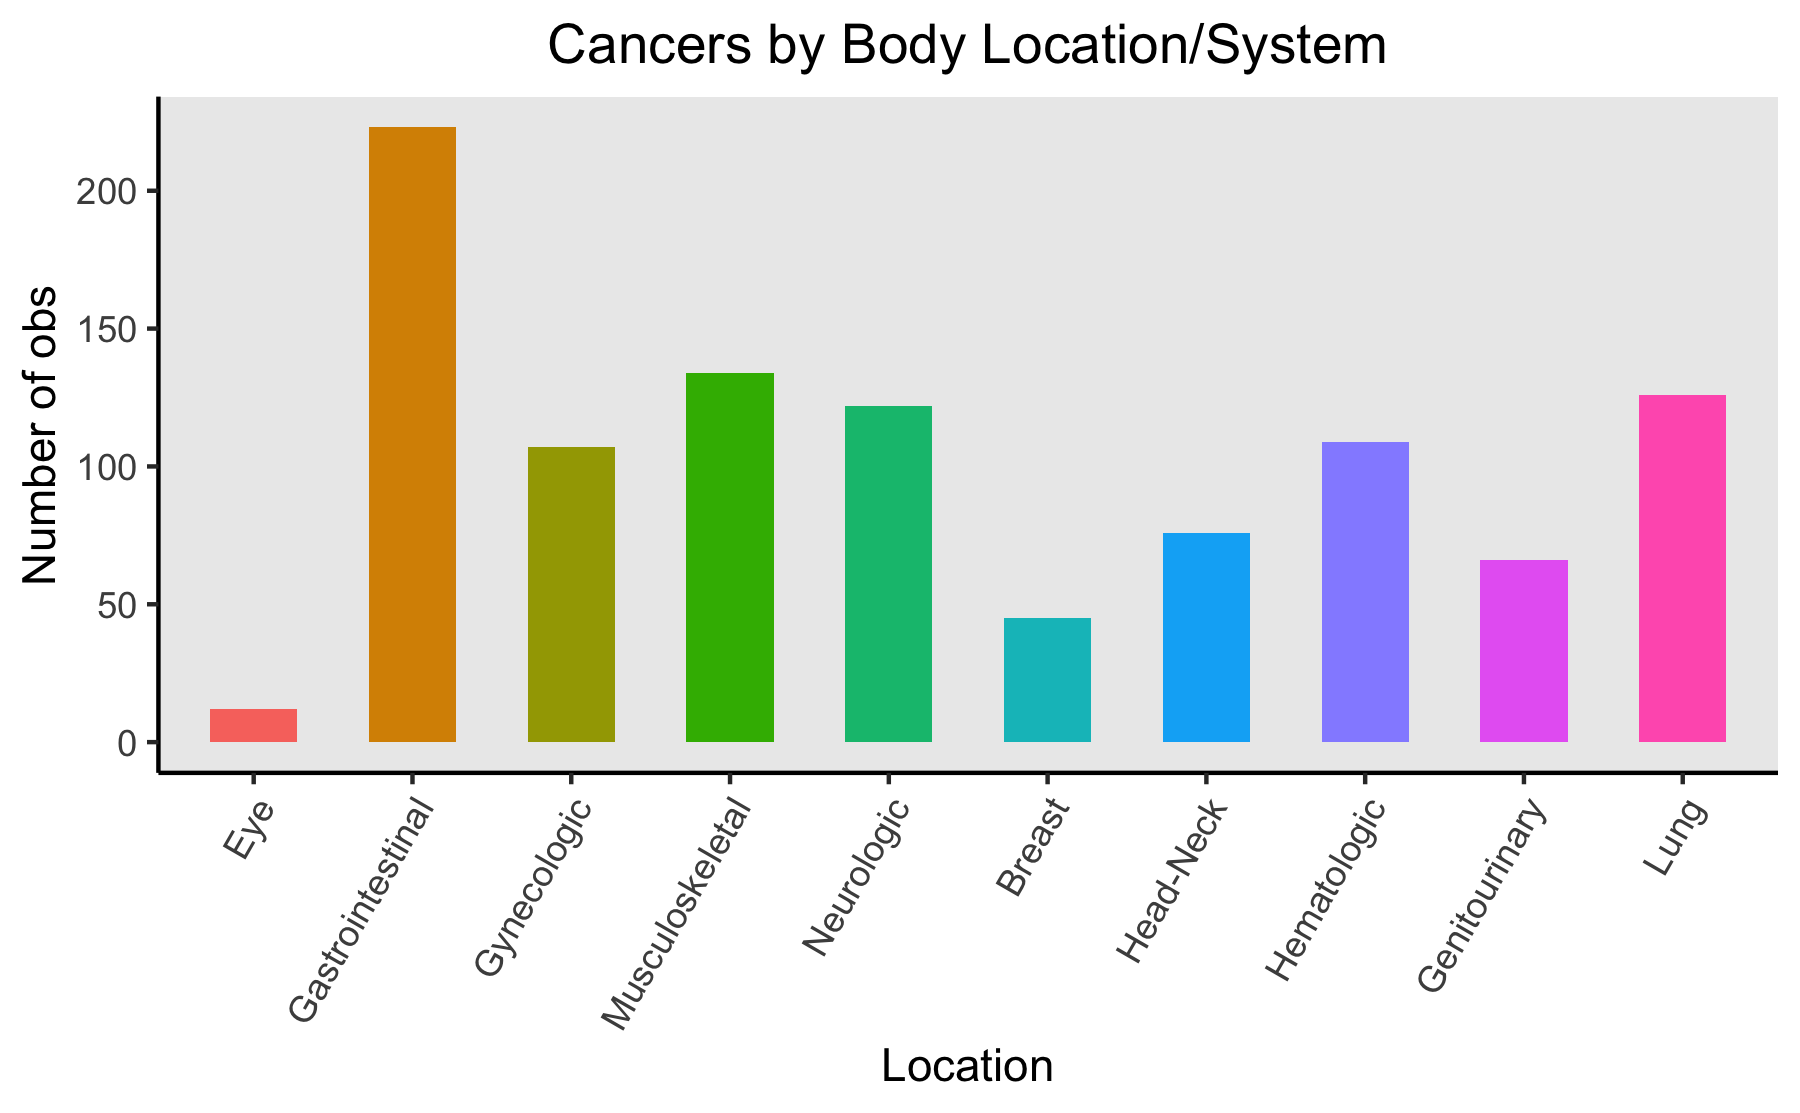
\includegraphics[width=0.65\textwidth]{plot1.png}
		\captionof{figure}{Cancer classes}\label{fig1}
	\end{wrapfigure}
	
	We hence grouped the various cancer types in 10 classes according to common medical knowledge\footnote{Cancer types grouped by body location: \url{https://www.cancer.gov/types/by-body-location}} and we obtained classes as reported in Figure \ref{fig1}.  "Eye" is the smallest one as there are only $16$ observations, $5$ of which labelled as "Enginereed". On the other hand, "Gastrointestinal" is the largest group and it comprehends $7$ types of cancer,  making this group quite heterogeneous.
	We decide to investigate two binary classification problems,  Blood vs Rest and Lung vs Rest, and the multiclass problem. We chose Lung because of the nature of such class: it is the most numerous group composed only by Lung cancer samples. The choice of Blood was instead driven by some underlying biological knowledge. In fact,  Blood cancer is quite different from other tumours because
	\begin{itemize}
		\item blood is in the whole body
		\item Leukemia, Lymphom and Myeloma are the main kinds of cancer but they all affect white blood cells
		\item not all blood cancers require a treatment, just periodical monitoring
	\end{itemize} 
	
	
	\section{Methods}
	\subsection{Random Forest}
	Whenever we are only interested in model performance and not in interpretability, Random Forest (RF) is a valid starting point. It frequently performs well on imbalanced data and it is a good compromise when working with correlated high-dimensional data. Furthermore, we can use Variable Importance of RFs to simply detect the most important features. This measure is calculated in three steps. First, prediction accuracy are measured on the out-of-bag samples. Then the values of the variable are randomly shuffled, keeping all other variables the same. Finally, the decrease in prediction accuracy on the shuffled data is measured and the mean decrease in accuracy across all trees is reported. Intuitively, the random shuffling means that, on average, the shuffled variable has no predictive power. This importance is a measure of by how much removing a variable decreases accuracy, and vice versa. \\
	We used this Variable Importance measure to select the most important feature in two different ways:
	%\begin{wrapfigure}{l}{0.3\textwidth}
	%	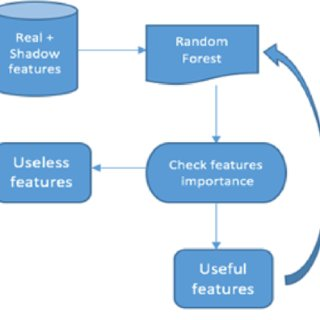
\includegraphics[width=0.3\textwidth]{Boruta-algo.jpg}\label{fig2}
	%\end{wrapfigure}
	
	\begin{itemize}
		\item \textit{Cross-validation}. We perfomed a 5-fold cross-validation on the model, selected the top most important features of each model and finally averaged.
		\item \textit{Boruta algorithm}\footnote{\url{https://www.researchgate.net/publication/220443685_Boruta_-_A_System_for_Feature_Selection}}: Boruta repeatedly measures feature importance then carries out statistical tests to screen out the features which are irrelevant. Here the steps:
		\begin{enumerate}
			\item Create copies of all the original features present in your dataset.
			\item Add randomness by shuffling these new feature. This is done to ensure that these new features show no correlation with the response variable.
			\item Run random forest classifier on the extended dataset and generate feature importance score based on mean accuracy decrease estimate for all the shadow variables.
			\item Compare Z-score of original variable with the maximum Z-score of shadow variables. Real features that have low score compared to the best of shadow features are deemed unimportant.
			\item Remove shadow features and repeat the process until an importance score is generated for all the variables.
		\end{enumerate}
	\end{itemize}
	
	
	\subsection{SVM-Lasso}
	Support vector machines (SVM) is based on the idea of finding a hyperplane that best separate classes. Here, we combine this method with a classical Lasso penalty, so that the objective function to be minimised is:
	\begin{equation*}
		\dfrac{1}{n} \sum_{i=1}^n hingeLoss(y_i(x_i w + t)) + \lambda \sum_{j=1}^p |w_j|  \qquad	\text{where} \qquad  hingeLoss(z) = max\{0, 1-z\}
	\end{equation*}
	Thus, we obtain the usual sparsity in predictors: some $w$ are shrunken all the way to zero and the remaining are the few relevant features.
	
	\subsection{Neural Networks}
	Nowadays, Neural Networks are a very attractive approach to obtain excellent performances.
	
	
	
	\section{Results}
	\subsection{Binary classifications}
	Before starting our Binary classifications on Blood and Lung cancer, we ran a Principal Component Analysis to gain some valuable insights. We noticed a surprising result: even if observations formed a cloud of points, Blood cancer cells were mainly concentrated in just one part of the 3-dimensional plot. The same did not happen for Lung cancer observations.
	
	We split the dataset into two parts, one used to train the model with all the features and select a small subset $(\sim 200)$ of them, the other to validate our model with only the selected features. The split was made with a ratio $(60:40)$ between first and second split and $(80:20)$ between training and test set in each split.
	The method used for selecting the features was different for RF and NN.
	
	We then moved to RF classifiers.  
	
	\subsubsection{Random Forests}
	
	\subsubsection{SVM-Lasso}
	
	\subsubsection{Neural Networks}
	
	
	\subsection{Multiclass classification}
	When working with the multiclass problem we decided to remove the group "Eye" because it was a small heterogeneous group that even after tuning for RF and NN held the worst accuracy scores. "Eye" was a cluster of different types of cancer: this didn't create problems when we were using a One vs All aproach but with multiclass the effects of doing the cluster ourselves was mor evident.  
	So after removing the group "Eye", we did the same as before and split the dataset in two.
	
	\subsubsection{Random Forests}
	We considered two different random forests, the first with the same parametes as the one used in Blood vs All random forest. Looking at the confusion matrix we can see hat most of the missclassification errors are data points classified as Gastrointestinal. Gastrointestinal was the biggest cluster we consider with a lot of different cancers so the genes( i.e. the features) important can be different within the cluster. To limit the weight of Gastrointestinal we decided to tune by hand the class weights. In this way we solve two problems: we reduced the importance of the group Gastrointestinal and we achieved at least one correct classification in each class. At this point we used cross validation to select five models and we extracted the most important features by looking at their relative importance in every model subjected to their presence in every model. We set a threshold to obtain  $(\sim 200)$ features and with this we created a reduced model that we fitted using the validation set we had created at the beginning.
	\subsubsection{SVM-Lasso}
	
	\subsubsection{Neural Networks}
	We first fitted a toy NN with only one hidden layer to see how the net worked.
	We then fitted three different NN: the first increasing by one the number of hidden layers, the second changing the loss function with the focal loss and the third using again the focal loss, but changing the alpha parameter w.r.t. the class percentage in the set.
	The three models held similar result with the second one being slightly more accurate. We the used the AWS console to perform feature importance because our computers were not sufficiently powerful to do that. (questa non so se metterla)
	
	\section{Overall Results}
	
	
	\section{Conclusion and future works}
	
	
	%\end{multicols}
\end{document}

\end{document}